% Источник: Leontiev-2017.pdf; печатная страница: 13; страница файла: 13
\section*{Глава I. Основные понятия и уравнения теории фильтрации}
\subsection*{§ 3. Законы сохранения массы и импульса при фильтрации в пористой среде}
\label{q2:sec-3}
\setcounter{footnote}{0}
Введенные в предыдущих параграфах функции от пространственных координат и времени --- $p(x^i,t)$, $\rho(x^i,t)$, $m(x^i,t)$ и $\boldsymbol{u}(x^i,t)$\footnote{В некоторых задачах, конечно, может потребоваться введение и других параметров, например температуры жидкости, концентрации примесей в ней и т.д.} --- заранее, вообще говоря, неизвестны и должны находиться на основе уравнений, выражающих универсальные законы сохранения, а также специальных физических закономерностей для конкретных изучаемых явлений (например, уравнений состояния или законов электродинамики). В простейших случаях
% Источник: Leontiev-2017.pdf; печатная страница: 14; страница файла: 14
для получения замкнутой системы дифференциальных уравнений оказывается достаточным использовать только два закона сохранения --- уравнения баланса массы и импульса, к феноменологическому описанию которых мы переходим.

\topic{Закон сохранения массы}
Интегральная формулировка закона сохранения массы жидкости получается из утверждения о том, что изменение массы жидкости в произвольном объеме $V$ внутри пористой среды происходит за счет притока жидкости через границу объема $\Sigma$:
\[
\frac{d}{dt}\int_V\rho m\,dV=-\int_\Sigma\rho\boldsymbol{u}\cdot\boldsymbol{n}\,d\sigma.
\]
Здесь $\boldsymbol{n}$ --- вектор внешней нормали к поверхности $\Sigma$ (из-за такого выбора нормали интеграл в правой части стоит со знаком минус), а объем $V$ неподвижен относительно пористой среды. Если входящие в это уравнение функции являются достаточно гладкими, то в левой части можно занести производную под знак интеграла, а правую часть преобразовать с помощью теоремы Гаусса--Остроградского:
\[
\int_V\frac{\partial(\rho m)}{\partial t}\,dV=-\int_V\Div(\rho\boldsymbol{u})\,dV,
\]
откуда в силу произвольности объема $V$ получается дифференциальная запись закона сохранения массы --- \textit{уравнение неразрывности}:
\begin{equation}
\frac{\partial(\rho m)}{\partial t}+\Div(\rho\boldsymbol{u})=0.
\tag{3.1}\label{q2:eq-3-1}
\end{equation}
Если плотность жидкости постоянна, а пористая среда не деформируется (т.е. пористость зависит только от координат), то первое слагаемое обращается в ноль и уравнение неразрывности приобретает вид
\begin{equation}
\Div\boldsymbol{u}=0.
\tag{3.2}\label{q2:eq-3-2}
\end{equation}

\topic{Уравнение баланса импульса --- закон Дарси}
Исторически уравнение баланса импульса было экспериментально получено французским гидравликом Анр\'и Дарс\'и (H.Darcy, 1856) для случая медленного стационарного движения несжимаемой жидкости в неподвижной изотропной пористой
% Источник: Leontiev-2017.pdf; печатная страница: 15; страница файла: 15
среде. В современных обозначениях это соотношение, называемое \textit{законом Дарси}, для фильтрации в поле тяжести имеет вид
\begin{equation}
0=-\grad p+\rho\boldsymbol{g}-\frac{\mu}{k}\boldsymbol{u},
\tag{3.3}\label{q2:eq-3-3}
\end{equation}
где $\boldsymbol{g}$ --- ускорение свободного падения, $\mu$ --- коэффициент динамической вязкости жидкости, $k$ --- коэффициент, называемый проницаемостью пористой среды, который зависит от типа пористой среды. По структуре уравнение \eqref{q2:eq-3-3} похоже на уравнение Навье--Стокса для вязкой несжимаемой жидкости при $\mu=\mathrm{const}$:
\begin{equation}
\rho\frac{d\boldsymbol{v}}{dt}=-\grad p+\rho\boldsymbol{g}+\mu\triangle\boldsymbol{v}
\tag{3.4}\label{q2:eq-3-4}
\end{equation}
и это не удивительно: макроскопический закон движения при фильтрации в пористой среде (закон Дарси) может быть получен с помощью некоторой процедуры осреднения из уравнения движения, описывающего внутрипоровое движение жидкости на микроуровне, то есть уравнения Навье--Стокса (см. § 5). При медленных (ползущих) течениях внутри пористой среды, для которых и справедлив закон Дарси, инерционные силы много меньше вязких сил, поэтому сто\'ящим в левой части \eqref{q2:eq-3-4} ускорением можно пренебречь, что даст при осреднении ноль в левой части \eqref{q2:eq-3-3}. Наличие же последнего слагаемого в \eqref{q2:eq-3-4}, описывающего действие вязкости, приводит при переходе к макроскопическому описанию к появлению объемной силы вязкого сопротивления, действующей на жидкость со стороны пористого скелета. В рассматриваемом случае медленных течений\setcounter{footnote}{0}\footnote{Более точно --- при числах Рейнольдса $\Rey=\rho vd/\mu\ll1$.} в изотропной среде сила сопротивления направлена противоположно скорости фильтрации, а ее величина прямо пропорциональна вязкости и модулю скорости фильтрации.

При $\boldsymbol{g}=0$ закон Дарси приобретает вид
\begin{equation}
\boldsymbol{u}=-\frac{k}{\mu}\grad p;
\tag{3.5}\label{q2:eq-3-5}
\end{equation}
знак минус в правой части \eqref{q2:eq-3-5} имеет ясный физический смысл: в отсутствие массовых сил жидкость движется в пористой среде из областей с б\'ольшим давлением в области с меньшим давлением.

% Источник: Leontiev-2017.pdf; печатная страница: 16; страница файла: 16
Если жидкость в порах покоится ($\boldsymbol{u}=0$), то закон Дарси превращается, как и следует, в обычное уравнение равновесия жидкости
\[
0=-\grad p+\rho\boldsymbol{g}.
\]

\topic{Коэффициент проницаемости}
\setcounter{footnote}{0}
Коэффициент проницаемости $k$ зависит только от свойств пористой среды (но не от свойств жидкости), и определяется, в основном, геометрией порового пространства. Он имеет размерность площади, а его величина имеет порядок квадрата характерного размера пор $d$\footnote{Для зависимости проницаемости от геометрических характеристик пористой среды предлагалось большое число приближенных формул, которые основаны на различных простых моделях внутрипорового пространства [16, 18]. В качестве примера приведем часто используемую формулу Козени--Кармана (J.Kozeny, P.C.Carman): $k\sim d^2m^3/(1-m)^2$, где характерный размер пор $d$ вычисляется как отношение объема образца к площади поверхности пор. Для плотной упаковки одинаковых сферических частиц диаметром $D$ справедлива приближенная формула $k=2\cdot10^{-3}D^2$.}. Для примера укажем, что типичные значения проницаемости для песчаников имеют порядок $10^{-15}$--$10^{-12}$~м$^2$, для почв --- $10^{-13}$--$10^{-11}$~м$^2$\footnote{Для сигареты $k\sim10^{-9}$~м$^2$.}.

В практических приложениях часто в качестве единицы $k$ выбирают такую проницаемость, чтобы в отсутствие тяжести (см. \eqref{q2:eq-3-5}) при градиенте давления\footnote{Килограмм-сила --- единица силы в технической системе единиц, приближенно равная весу эталона килограмма у поверхности земли: $1$~кгс $=9{,}80665$~Н $\approx9{,}81$~Н.} $1$~кгс/см$^3\approx1$~атм/см жидкость с вязкостью $0{,}01$~г/(см$\cdot$с) (вязкость воды при $20^\circ$C) имела скорость фильтрации $1$~см/с. Эта единица проницаемости называется \textit{дарси} (обозначение «Д»); $1$~Д $\approx1{,}02\cdot10^{-12}$~м$^2\approx1$~мкм$^2$.

Для неоднородных пористых сред коэффициент проницаемости является функцией пространственных координат и может меняться с течением времени (например, при деформациях пористого скелета или за счет его засорения или растворения).

\topic{Коэффициент фильтрации}
В гидротехнической практике закон Дарси обычно используется в виде уравнения, разрешенного относительно скорости фильтрации, причем вместо давления используется
% Источник: Leontiev-2017.pdf; печатная страница: 17; страница файла: 17
\textit{пьезометрический напор} (или просто \textit{напор})\setcounter{footnote}{0}\footnote{Напор имеет размерность длины и с точностью до постоянного слагаемого равен вертикальной координате свободной поверхности жидкости в измерительной скважине, пробуренной в пористый пласт, чем и объясняется удобство его использования.}
\[
H=H(x,y,z,t)=\frac{p}{\rho g}+z,
\]
где $z$ --- вертикальная координата рассматриваемой точки (ось $Oz$ направлена вверх, противоположно $\boldsymbol{g}$). Выразив скорость фильтрации из \eqref{q2:eq-3-3}, получим
\begin{equation}
\boldsymbol{u}=-C\grad H,\qquad C=\frac{k\rho g}{\mu},
\tag{3.6}\label{q2:eq-3-6}
\end{equation}
где $C$ --- \textit{коэффициент фильтрации}, зависящий, очевидно, как от свойств пористой среды, так и от свойств жидкости\footnote{В англоязычной литературе величину $C$ обычно называют «гидравлической проводимостью» (\textit{hydraulic conductivity}).}. Типичные значения $C$ при фильтрации воды в песке имеют порядок $10^{-5}$--$10^{-2}$~м/с, в почве --- $10^{-6}$--$10^{-4}$~м/с, в глине --- $10^{-7}$--$10^{-6}$~м/с.

\topic{Закон Дарси для анизотропных сред}
При фильтрации в анизотропных пористых средах (например, в осадочных слоистых пластах или в средах с трещинами, направленными в выделенном направлении) линейная зависимость скорости фильтрации и градиента давления сохраняется (для медленных течений), однако эти векторы в случае общего положения уже не будут параллельны. Проницаемость таких сред будет характеризоваться не одним числом (коэффициентом проницаемости $k$), а симметричным положительно-определенным \textit{тензором проницаемости} $k_{ij}$, входящим в закон Дарси
\[
u_i=-\frac{k_{ij}}{\mu}(\nabla^jp-\rho g^j).
\]
Например, в слоистой среде, у которой направление, перпендикулярное плоскости напластования, задается единичным вектором $\boldsymbol{n}$, тензор проницаемости в декартовой системе координат имеет вид
\[
k_{ij}=(k_\perp-k_\parallel)n_in_j+k_\parallel\delta_{ij},
\]
где $k_\perp$ и $k_\parallel$ суть проницаемости при фильтрации соответственно поперек и вдоль напластования.

% Источник: Leontiev-2017.pdf; печатная страница: 18; страница файла: 18
\subsection*{§ 4. Законы фильтрации, отличные от закона Дарси}
\label{q2:sec-4}
\topic{Пределы применимости закона Дарси}
\setcounter{footnote}{0}
В некоторых практически важных ситуациях при фильтрации жидкостей --- речь идет об однородных жидкостях, целиком заполняющих недеформируемые изотропные пористые среды --- наблюдаются отступления от классического закона Дарси \eqref{q2:eq-3-3}. Эти отклонения связаны с двумя причинами. \textit{Первая} --- это немалость скоростей движения жидкости внутри пор, т.е. невозможность пренебречь инерционными членами в микроскопических уравнениях \eqref{q2:eq-3-4}. Такие условия, в которых неприменимо приближение Стокса, возникают, например, в прискважинных областях или при фильтрации в крупнозернистых пористых средах (фильтрация через гравий и гальку, а также через гранулированные среды в промышленных технологических установках). \textit{Вторая} причина состоит в отличии реологических\footnote{Реология --- наука, изучающая связи между напряжениями и деформационными характеристиками материалов. Название науки, предложенное американским исследователем Ю.Бингамом (E.Bingham, 1920), происходит от греческого $\rho\varepsilon\omega$ --- «теку», «струюсь».} соотношений фильтрующейся жидкости от закона Навье--Стокса, причем неньютоновское поведение жидкостей при течении внутри порового пространства может проявляться как в узкой пристеночной области (за счет физико-химического взаимодействия жидкости со стенкой поры), так и во всем объеме жидкости (например, при фильтрации некоторых нефтей).

\topic{Вид закона фильтрации при немалых скоростях фильтрации}
Предполагая для простоты, что массовые силы отсутствуют\footnote{Влияние потенциальных сил можно учесть путем переопределения давления (например, в случае фильтрации несжимаемой однородной жидкости в поле силы тяжести --- с помощью введения новой переменной $p'=p-\rho\boldsymbol{r}\cdot\boldsymbol{g}$, где $\boldsymbol{r}$ --- радиус-вектор).}, установим общий вид зависимости градиента давления от скорости фильтрации с использованием теории размерностей.

Модуль градиента давления $|\grad p|$ при стационарной фильтрации зависит, кроме модуля скорости фильтрации $u$, от свойств жидкости (плотности $\rho$ и вязкости $\mu$) и пористой среды (характерного размера пор $d$, пористости $m$ и, возможно, других скалярных безразмерных параметров $a_\alpha$, определяющих геометрию
% Источник: Leontiev-2017.pdf; печатная страница: 19; страница файла: 19
порового пространства):
\[
|\grad p|=F(u,\rho,\mu,d,m,a_\alpha),
\]
и применение $\pi$-теоремы [6,15] дает зависимость
\[
|\grad p|=\frac{\mu u}{d^2}\cdot\Phi(\Rey,m,a_\alpha),\qquad \Rey=\frac{\rho ud}{\mu}.
\]
Что касается направления вектора $\grad p$, то, как нетрудно видеть, он должен быть параллелен вектору $\boldsymbol{u}$. В самом деле, в прямоугольной декартовой системе координат зависимость компонент вектора $\grad p$ от компонент вектора скорости фильтрации $\boldsymbol{u}$ и других определяющих параметров имеет вид
\[
\nabla_kp=\varphi_k(u_j,\rho,\mu,d,m,a_\alpha),
\]
причем вид функций $\varphi_k$ не зависит от выбора системы координат. Предположим, что векторы $\grad p$ и $\boldsymbol{u}$ не параллельны. Направим ось $Ox$ вдоль вектора $\boldsymbol{u}$, так чтобы он имел только одну отличную от нуля компоненту. Тогда при повороте системы координат относительно оси $Ox$ все аргументы функций $\varphi_k$ останутся неизменными, в то время как компоненты вектора $\grad p$ будут изменяться, что приводит к противоречию. Отметим, что это рассуждение неявно опирается на предположение об \textit{изотропности} пористой среды. Для \textit{анизотропных} сред (в которых, конечно, векторы $\boldsymbol{u}$ и $\grad p$ могут быть не параллельны) в число аргументов функций $\varphi_k$ нужно дополнительно включать компоненты тензоров, характеризующих анизотропию\setcounter{footnote}{0}\footnote{Например, для слоистой среды --- компоненты вектора нормали $\boldsymbol{n}$ к плоскости напластования (см. с. 17).}.

Итак, общий вид закона фильтрации несжимаемой жидкости в изотропной пористой среде можно записать так:
\begin{equation}
\grad p=-\frac{\mu\boldsymbol{u}}{d^2}\Phi(\Rey,m,a_\alpha).
\tag{4.1}\label{q2:eq-4-1}
\end{equation}
Зависимость $\Phi(\Rey)$ в двух предельных случаях --- при малых и больших числах Рейнольдса --- можно установить из общих соображений.

В случае \textit{очень медленных} (ползущих) внутрипоровых течений, в которых доминируют вязкие эффекты, зависимость \eqref{q2:eq-4-1}
% Источник: Leontiev-2017.pdf; печатная страница: 20; страница файла: 20
не должна содержать плотность жидкости, выпадающую из уравнений вязкой жидкости в приближении Стокса. Поэтому при $\Rey\ll1$ функция $\Phi$ не должна зависеть от числа Рейнольдса, и закон фильтрации \eqref{q2:eq-4-1} можно записать в виде
\[
\grad p=-\frac{\mu}{k}\boldsymbol{u},\quad k=\frac{d^2}{\Phi(0,m,a_\alpha)},
\]
где величина $k$, имеющая размерность квадрата длины и зависящая только от свойств пористой среды, должна, в силу закона Дарси \eqref{q2:eq-3-5}, совпадать с коэффициентом проницаемости.

\setcounter{figure}{4}
\begin{figure}[H]
\centering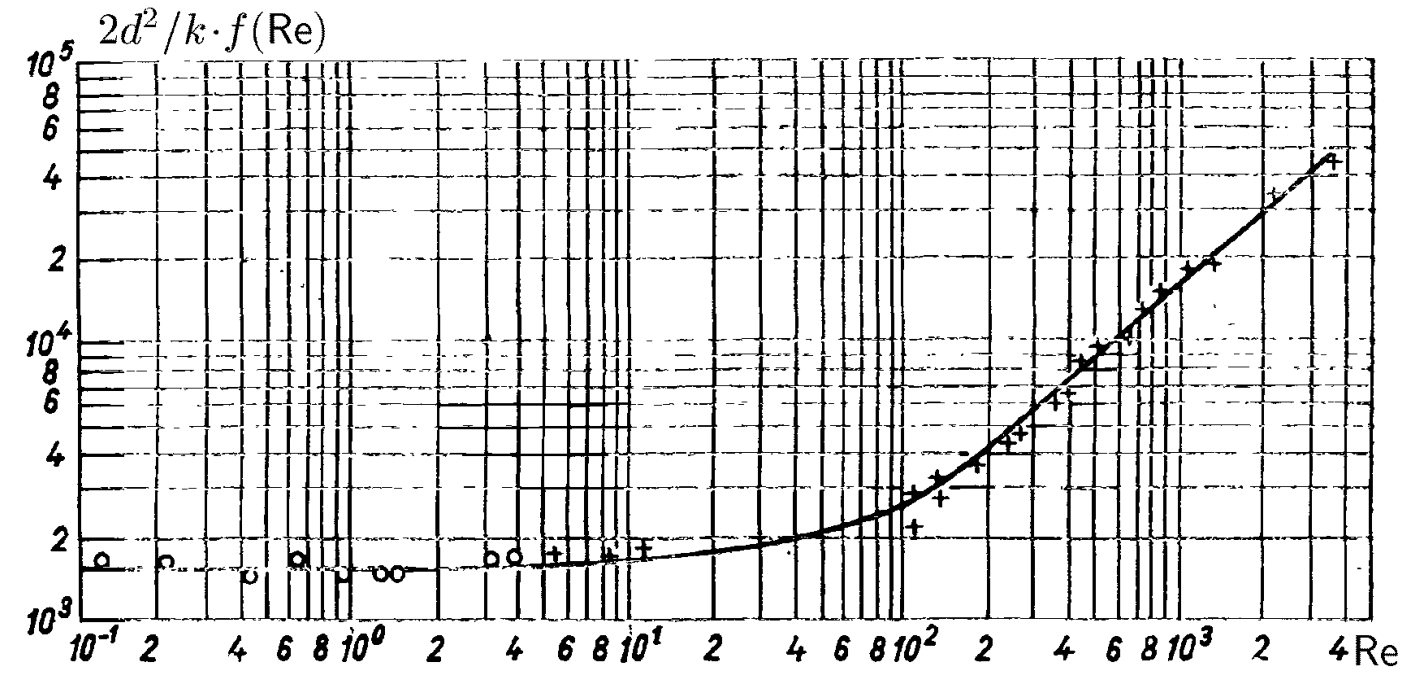
\includegraphics[width=.95\linewidth]{figures/figure-5.png}
\caption{}\label{q2:fig-5}
\end{figure}
В противоположном случае \textit{быстрых внутрипоровых течений} (при $\Rey\gg1$) преобладающими должны быть инерционные эффекты, поэтому зависимость градиента давления от скорости фильтрации не должна содержать в главных членах коэффициент вязкости $\mu$. Это дает при больших $\Rey$ линейную зависимость $\Phi(\Rey)$ и квадратичную зависимость $|\grad p|$ от $u$.

Если нормировать функцию $\Phi(\Rey)$, вводя обозначение
\begin{equation}
f(\Rey)=\Phi(\Rey)/\Phi(0),\quad f(0)=1,\quad f(\Rey)=O(\Rey)\text{ при }\Rey\to\infty,
\tag{4.2}\label{q2:eq-4-2}
\end{equation}
то закон фильтрации в принимает окончательный вид
% Сохранена опечатка оригинала: «то закон фильтрации в принимает».
\[
0=-\grad p+\rho\boldsymbol{g}-\frac{\mu}{k}\boldsymbol{u}\cdot f(\Rey),\quad \Rey=\frac{\rho ud}{\mu}.
\]
Пример зависимости $f(\Rey)$, полученной экспериментально для нескольких пористых сред [5], показан на рис.~\ref{q2:fig-5} (величина $f$
% Источник: Leontiev-2017.pdf; печатная страница: 21; страница файла: 21
умножена на безразмерный коэффициент $2d^2/k$; шкалы на обеих осях логарифмические).

\topic{Двучленный закон фильтрации}
При практических расчетах закон $f(\Rey)$ часто аппроксимируют линейной зависимостью, удовлетворяющей требованиям \eqref{q2:eq-4-2}:
\[
f(\Rey)=1+\frac{\beta\sqrt{k}}{d}\Rey,
\]
где $\beta$ --- безразмерный параметр, зависящий от структуры пористой среды (порядка единицы). Это дает \textit{двучленный закон фильтрации}, называемый также \textit{законом фильтрации Форхгеймера} (P.Forchheimer, 1901):
\begin{equation}
0=-\grad p+\rho\boldsymbol{g}-\frac{\mu}{k}\boldsymbol{u}-\beta\frac{\rho u^2}{\sqrt{k}}\cdot\frac{\boldsymbol{u}}{u}.
\tag{4.3}\label{q2:eq-4-3}
\end{equation}

\topic{О «турбулентном» режиме фильтрации}
Как видно из рис.~\ref{q2:fig-5}, отклонения от закона Дарси, которому соответствует горизонтальный участок графика, начинаются при $\Rey$ порядка единиц (числа Рейнольдса вычисляются по характерному размеру зерен). При дальнейшем повышении скорости фильтрации инерцией жидкости при ее движении в извилистом внутрипоровом пространстве уже нельзя пренебрегать и нужно пользоваться, например, квадратичной зависимостью \eqref{q2:eq-4-3}. Этот закон по своей структуре (квадратичная зависимость от скорости) похож на известную связь сопротивления и скорости при развитом турбулентном движении жидкости в каналах или при обтекании тел потоком. Основываясь на этой формальной аналогии, иногда режим фильтрации в области применимости закона \eqref{q2:eq-4-3} называют «турбулентной фильтрацией». В действительности же, как показывают эксперименты, при переходе через границу применимости закона Дарси движение жидкости в порах остается ламинарным, а переход к турбулентности происходит при достаточно больших числах Рейнольдса (около 100--300).

\topic{Фильтрация неньютоновских жидкостей}
Отклонения от закона Дарси, связанные с неньютоновскими свойствами жидкости, могут иметь различный характер в зависимости от реологического поведения чистой жидкости.

% Источник: Leontiev-2017.pdf; печатная страница: 22; страница файла: 22
\setcounter{footnote}{0}
Ряд веществ, например растворы полимеров, при простом сдвиге --- течении с полем скорости $\boldsymbol{v}=(v_x(y);0;0)$ --- имеет \textit{степенн\'ую зависимость} касательных напряжений от скорости сдвига:
\[
\tau_{xy}\sim(e_{xy})^n,
\]
где $n$ --- некоторая константа\footnote{Например, для зубной пасты «Колгейт» $n\approx0{,}2$, для шоколада в жидком состоянии $n\approx0{,}6$.}; значение $n=1$ соответствует обычной ньютоновской жидкости. При течении таких сред в цилиндрическом капилляре радиуса $R$ зависимость скорости от радиальной координаты задается степенной функцией, а связь расхода и градиента давления вдоль капилляра описывается соотношением
\[
Q\sim R^{(3n+1)/n}|\grad p|^{1/n},
\]
переходящим при $n=1$ в закон Пуазейля. Если в качестве простейшей модели пористой среды рассмотреть пучок параллельных капилляров с некоторым распределением радиусов (рис. 4), то из предыдущей формулы получается \textit{степенной закон фильтрации}
\[
\boldsymbol{u}=-A\,|\grad p|^{\frac{1}{n}-1}\cdot\grad p,\qquad A=\mathrm{const}.
\]
При фильтрации некоторых высокомолекулярных соединений становятся существенными релаксационные эффекты, проявляющиеся, например, в запаздывании изменения скорости фильтрации при изменении градиента давления и т.п. Для описания таких фильтрационных процессов часто используются различные эвристические модели, в которых между скоростью фильтрации и градиентом давления имеется не алгебраическая, а дифференциальная связь. Примером такой модели служит закон фильтрации
\[
\grad p+\tau_p\frac{\partial\grad p}{\partial t}=-\frac{\mu}{k}\left(\boldsymbol{u}+\tau_u\frac{\partial\boldsymbol{u}}{\partial t}\right),
\]
где константы $\tau_p$ и $\tau_u$ имеют смысл времен релаксации давления и скорости фильтрации.

В ряде природных процессов, например при просачивании воды в мелкопористых средах или при фильтрации некоторых нефтей, течение жидкости начинается при превышении модулем градиента давления $|\grad p|$ некоторого фиксированного порогового
% Источник: Leontiev-2017.pdf; печатная страница: 23; страница файла: 23
значения $G$ («предельного градиента»), а при меньших градиентах жидкость в порах покоится\setcounter{footnote}{0}\footnote{Отметим для сравнения, что при выполнении закона Дарси фильтрационное течение начинается при любых сколь угодно малых градиентах давления.}. В качестве примеров таких законов фильтрации на рис.~\ref{q2:fig-6} показаны экспериментальные зависимости скорости фильтрации от градиента давления для воды в глинизированном песчанике (\textit{а}) и нефти в песке (\textit{б}), заимствованные из [2]. Изучение особенностей подобных законов важно при разработке нефтяных месторождений, т.к. большая часть пласта приходится как раз на области малых градиентов.

\begin{figure}[H]
\centering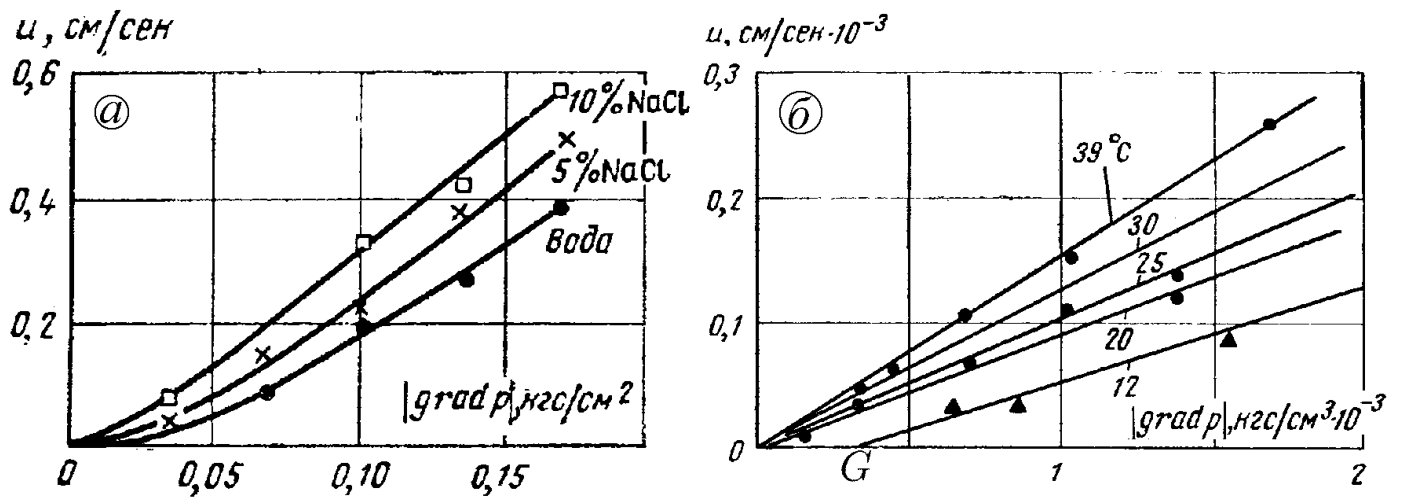
\includegraphics[width=.95\linewidth]{figures/figure-6.png}
\caption{}\label{q2:fig-6}
\end{figure}
Для моделирования таких явлений часто используется \textit{закон фильтрации с предельным (начальным) градиентом}
\begin{equation}
\boldsymbol{u}=\begin{cases}
-\dfrac{k}{\mu}(|\grad p|-G)\cdot\dfrac{\grad p}{|\grad p|}&\text{при }|\grad p|\geqslant G,\\[6pt]
0&\text{при }|\grad p|<G.
\end{cases}
\tag{4.4}\label{q2:eq-4-4}
\end{equation}
Особенностью этой модели является возможность существования застойных зон (с нулевой скоростью фильтрации), в которых давление не определено однозначно и зависит от предыстории течения.

Наличие предельного градиента легко объяснить, если предположить, что фильтрующаяся жидкость проявляет \textit{вязкопластические свойства} (т.е. начинает течь лишь тогда, когда интенсивность касательных напряжений --- функция от второго инварианта девиатора тензора напряжений --- достигает фиксированного ненулевого значения). Например, жидкость Бингама--Шведова,
% Источник: Leontiev-2017.pdf; печатная страница: 24; страница файла: 24
которая при простом сдвиге описывается соотношениями
\[
e_{xy}=\begin{cases}
\dfrac{1}{2\mu}(|\tau_{xy}|-\tau_0)\cdot\dfrac{\tau_{xy}}{|\tau_{xy}|}&\text{при }|\tau_{xy}|\geqslant\tau_0,\\[6pt]
0&\text{при }|\tau_{xy}|<\tau_0,
\end{cases}
\]
начинает движение в цилиндрическом капилляре радиуса $R$ при превышении градиентом давления значения $|\grad p|=2\tau_0/R$ ($\tau_0$ --- пороговое касательное напряжение)\setcounter{footnote}{0}\footnote{Уточним, что в движение приходит пристеночный слой жидкости; в центральной части капилляра при любых, даже очень больших градиентах некоторая часть жидкости движется как твердое тело.}. При моделировании пористой среды набором параллельных каналов с различными радиусами отсюда получается закон фильтрации, качественно схожий с \eqref{q2:eq-4-4}, причем предельный градиент определяется радиусом наибольшего капилляра.
% Конец § 4. Следующий заголовок оригинала: § 5. Вывод дифференциальных уравнений фильтрации с помощью осреднения микроскопических уравнений.
